\section{Vergleich}
\begin{figure}
    \centering
    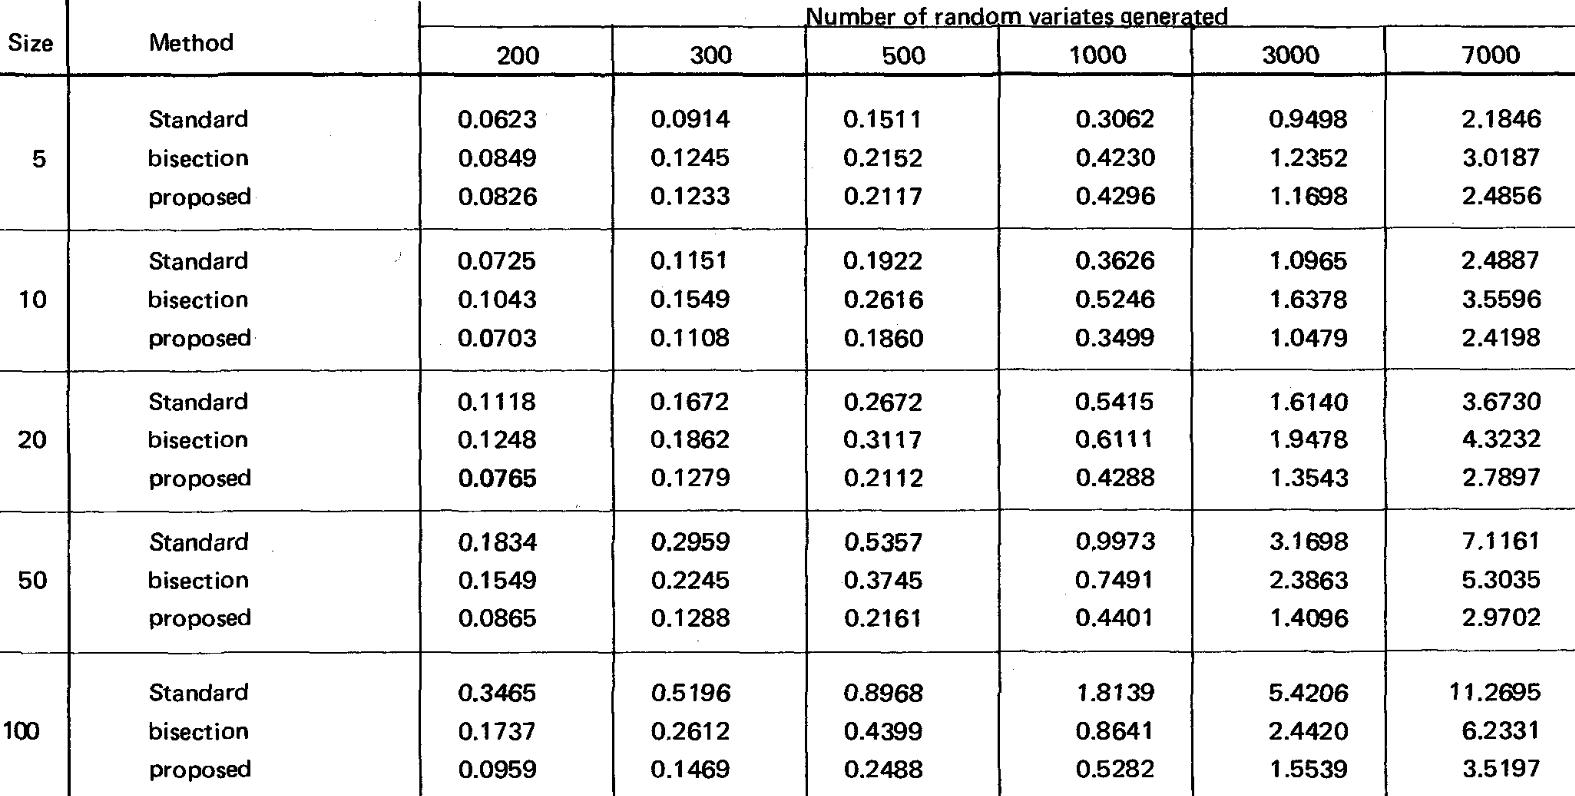
\includegraphics[width=0.48\textwidth]{Screenshots/chenAsauHashTableComp.png}
    \caption{Laufzeiten unterschiedlicher Algorithmen: Standard (\eqref{eq:hash_ineq} 
        wird trivial berechnet), Bisection (\eqref{eq:hash_ineq} wird mit einfacher 
        binarär Suche berechnet) und Proposed (die vorgestellte Methode mit 
        Indextabelle). Auszug aus Chen und Asau \cite{chen_asau-generating_random_variates-1974}.}
    \label{fig:computationTimeComp}
\end{figure}
Chen und Asau haben in ihrer Arbeit über die hash-basierte Inversionsmethode 
gezeigt, dass ihre Methode für große Zahlen um eine Magnitude schneller ist, 
als triviale Methoden. Durch den Einsatz der Hashtabelle werden, anstelle von 
$O(n)$ Berechnungen wie bei der trivialsten Methode lineare Suche oder $O(\log
(n))$ Berechnungen bei binärer Suche, bei gut gewählter Größe der Hashtabelle 
nur noch $O(1)$ Berechnungen je Zufallsvariable durchgeführt. Diese Verbesserung 
hängt mit der 
Eigenschaft von Arrays und Hashtabellen zusammen, auf jedes Element in $O(1)$ 
zugreifen zu können. Deshalb kann die hashbasierte Inversionsmethode ihre 
Stärken erst bei vielen zu überprüfenden Intervallen, und damit Einträgen in 
der Tabelle, ausspielen. In Chen und Asau's Tests sieht man, das für wenige 
Intervalle ($5$) die Hashtabelle langsamer ist als triviales Testen der 
Ungleichungen. Mit $100$ Einträgen ist die vorgestellte Methode aber schon mehr 
als $3$-mal so schnell wie herkömmliche Verfahren. Das liegt daran, dass bei 
wenigen Intervallen die Initialisierung der Hashtabelle einen sog. Overhead 
erschafft, da der Aufwand, sie mit Werten zu befüllen und alle Möglichkeiten 
vorher zu berechnen, nicht durch viele Zugriffe wieder gutgemacht wird.

Wie in der Einleitung benannt, gibt es noch die Möglichkeit, Huffman-Bäume 
einzusetzen. Diese kodieren Werte nach ihrer Häufigkeit, wodurch häufig 
vorkommende Werte kürzer dargestellt werden und dadurch weniger Platz, verbrauchen. 
Diese Bäume können auch traversiert werden, wobei auch hier der kürzere Weg für 
häufigere Werte von Vorteil ist. Es ist möglich, einen solchen Baum abzuwandeln, 
damit er sinnvoll in der Partialsummenberechnung eingesetzt werden kann. Dadurch 
ergeben sich optimale Laufzeiten, die durch konstante Werte je nach Implementierung 
sogar besser als jene einer Hashtabelle sein können. In dieser Arbeit werden 
allerdings keine Vergleiche gezeigt, da die Implementierung eines Huffman-Baumes 
über den Rahmen dieser Ausarbeitung hinausgehen würde.

Durch die Hashtabelle werden bei sehr großen Mengen an Zufallsvariablen viele 
komplizierte Berechnungen gespart, da nur bei der Initialisierung die 
möglicherweise aufwändige Invertierung berechnet wird. Durch das Zusammenfallen 
von Werten durch nur endlich viele Einträge in der Hashtabelle, eignet sich die 
hashbasierte Inversion allerdings nur, wenn die Berechnung und Auswertung der 
Dichtefunktion sehr aufwändig ist und man nicht die Ressourcen oder Zeit besitzt, 
diese für jeden Wert auszuführen.

